% Name: R-move, time going down
% Description: The same R-move read from top to bottom: a and b enter at the top, a crosses in front of b, and they fuse into c below.
% Tags: R-move, R-symbol, braiding, anyons, time going down

$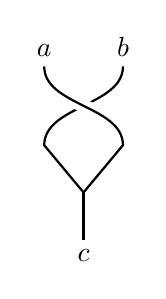
\begin{tikzpicture}[thick, baseline=(current bounding box.center)]
  \draw (1,2.2) node[above] {$b$} .. controls (1,1.7) and (0,1.7) .. (0,1.2) -- (0.5,0.6);
  \draw[white, line width=5pt] (0,2.2) .. controls (0,1.7) and (1,1.7) .. (1,1.2);
  \draw (0,2.2) node[above] {$a$} .. controls (0,1.7) and (1,1.7) .. (1,1.2) -- (0.5,0.6);
  \draw (0.5,0.6) -- (0.5,0) node[below] {$c$};
\end{tikzpicture}
\;=\; R^{ab}_c
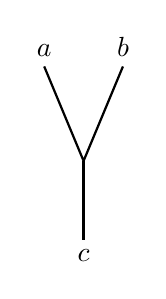
\begin{tikzpicture}[thick, baseline=(current bounding box.center)]
  \draw (0,2.2) node[above] {$a$} -- (0.5,1) -- (1,2.2) node[above] {$b$};
  \draw (0.5,1) -- (0.5,0) node[below] {$c$};
\end{tikzpicture}$
